% Options for packages loaded elsewhere
\PassOptionsToPackage{unicode}{hyperref}
\PassOptionsToPackage{hyphens}{url}
\PassOptionsToPackage{dvipsnames,svgnames,x11names}{xcolor}
%
\documentclass[
  letterpaper,
  DIV=11,
  numbers=noendperiod]{scrartcl}

\usepackage{amsmath,amssymb}
\usepackage{iftex}
\ifPDFTeX
  \usepackage[T1]{fontenc}
  \usepackage[utf8]{inputenc}
  \usepackage{textcomp} % provide euro and other symbols
\else % if luatex or xetex
  \usepackage{unicode-math}
  \defaultfontfeatures{Scale=MatchLowercase}
  \defaultfontfeatures[\rmfamily]{Ligatures=TeX,Scale=1}
\fi
\usepackage{lmodern}
\ifPDFTeX\else  
    % xetex/luatex font selection
\fi
% Use upquote if available, for straight quotes in verbatim environments
\IfFileExists{upquote.sty}{\usepackage{upquote}}{}
\IfFileExists{microtype.sty}{% use microtype if available
  \usepackage[]{microtype}
  \UseMicrotypeSet[protrusion]{basicmath} % disable protrusion for tt fonts
}{}
\makeatletter
\@ifundefined{KOMAClassName}{% if non-KOMA class
  \IfFileExists{parskip.sty}{%
    \usepackage{parskip}
  }{% else
    \setlength{\parindent}{0pt}
    \setlength{\parskip}{6pt plus 2pt minus 1pt}}
}{% if KOMA class
  \KOMAoptions{parskip=half}}
\makeatother
\usepackage{xcolor}
\setlength{\emergencystretch}{3em} % prevent overfull lines
\setcounter{secnumdepth}{-\maxdimen} % remove section numbering
% Make \paragraph and \subparagraph free-standing
\ifx\paragraph\undefined\else
  \let\oldparagraph\paragraph
  \renewcommand{\paragraph}[1]{\oldparagraph{#1}\mbox{}}
\fi
\ifx\subparagraph\undefined\else
  \let\oldsubparagraph\subparagraph
  \renewcommand{\subparagraph}[1]{\oldsubparagraph{#1}\mbox{}}
\fi


\providecommand{\tightlist}{%
  \setlength{\itemsep}{0pt}\setlength{\parskip}{0pt}}\usepackage{longtable,booktabs,array}
\usepackage{calc} % for calculating minipage widths
% Correct order of tables after \paragraph or \subparagraph
\usepackage{etoolbox}
\makeatletter
\patchcmd\longtable{\par}{\if@noskipsec\mbox{}\fi\par}{}{}
\makeatother
% Allow footnotes in longtable head/foot
\IfFileExists{footnotehyper.sty}{\usepackage{footnotehyper}}{\usepackage{footnote}}
\makesavenoteenv{longtable}
\usepackage{graphicx}
\makeatletter
\def\maxwidth{\ifdim\Gin@nat@width>\linewidth\linewidth\else\Gin@nat@width\fi}
\def\maxheight{\ifdim\Gin@nat@height>\textheight\textheight\else\Gin@nat@height\fi}
\makeatother
% Scale images if necessary, so that they will not overflow the page
% margins by default, and it is still possible to overwrite the defaults
% using explicit options in \includegraphics[width, height, ...]{}
\setkeys{Gin}{width=\maxwidth,height=\maxheight,keepaspectratio}
% Set default figure placement to htbp
\makeatletter
\def\fps@figure{htbp}
\makeatother

\KOMAoption{captions}{tableheading,figureheading}
\makeatletter
\makeatother
\makeatletter
\makeatother
\makeatletter
\@ifpackageloaded{caption}{}{\usepackage{caption}}
\AtBeginDocument{%
\ifdefined\contentsname
  \renewcommand*\contentsname{Tabla de contenidos}
\else
  \newcommand\contentsname{Tabla de contenidos}
\fi
\ifdefined\listfigurename
  \renewcommand*\listfigurename{Listado de Figuras}
\else
  \newcommand\listfigurename{Listado de Figuras}
\fi
\ifdefined\listtablename
  \renewcommand*\listtablename{Listado de Tablas}
\else
  \newcommand\listtablename{Listado de Tablas}
\fi
\ifdefined\figurename
  \renewcommand*\figurename{Figura}
\else
  \newcommand\figurename{Figura}
\fi
\ifdefined\tablename
  \renewcommand*\tablename{Tabla}
\else
  \newcommand\tablename{Tabla}
\fi
}
\@ifpackageloaded{float}{}{\usepackage{float}}
\floatstyle{ruled}
\@ifundefined{c@chapter}{\newfloat{codelisting}{h}{lop}}{\newfloat{codelisting}{h}{lop}[chapter]}
\floatname{codelisting}{Listado}
\newcommand*\listoflistings{\listof{codelisting}{Listado de Listados}}
\makeatother
\makeatletter
\@ifpackageloaded{caption}{}{\usepackage{caption}}
\@ifpackageloaded{subcaption}{}{\usepackage{subcaption}}
\makeatother
\makeatletter
\@ifpackageloaded{tcolorbox}{}{\usepackage[skins,breakable]{tcolorbox}}
\makeatother
\makeatletter
\@ifundefined{shadecolor}{\definecolor{shadecolor}{rgb}{.97, .97, .97}}
\makeatother
\makeatletter
\makeatother
\makeatletter
\makeatother
\ifLuaTeX
\usepackage[bidi=basic]{babel}
\else
\usepackage[bidi=default]{babel}
\fi
\babelprovide[main,import]{spanish}
% get rid of language-specific shorthands (see #6817):
\let\LanguageShortHands\languageshorthands
\def\languageshorthands#1{}
\ifLuaTeX
  \usepackage{selnolig}  % disable illegal ligatures
\fi
\usepackage[]{biblatex}
\addbibresource{../../../../references.bib}
\IfFileExists{bookmark.sty}{\usepackage{bookmark}}{\usepackage{hyperref}}
\IfFileExists{xurl.sty}{\usepackage{xurl}}{} % add URL line breaks if available
\urlstyle{same} % disable monospaced font for URLs
\hypersetup{
  pdftitle={Abordando el cambio climático y otros desafíos ambientales Perspectivas y soluciones},
  pdfauthor={Edison Achalma},
  pdflang={es},
  colorlinks=true,
  linkcolor={blue},
  filecolor={Maroon},
  citecolor={Blue},
  urlcolor={Blue},
  pdfcreator={LaTeX via pandoc}}

\title{Abordando el cambio climático y otros desafíos ambientales
Perspectivas y soluciones}
\usepackage{etoolbox}
\makeatletter
\providecommand{\subtitle}[1]{% add subtitle to \maketitle
  \apptocmd{\@title}{\par {\large #1 \par}}{}{}
}
\makeatother
\subtitle{Explorando el impacto, mitigación y adaptación al cambio
climático, reformas inclusivas y análisis de productos tradicionales y
recursos naturales}
\author{Edison Achalma}
\date{2022-06-03}

\begin{document}
\maketitle
\ifdefined\Shaded\renewenvironment{Shaded}{\begin{tcolorbox}[borderline west={3pt}{0pt}{shadecolor}, enhanced, interior hidden, sharp corners, breakable, boxrule=0pt, frame hidden]}{\end{tcolorbox}}\fi

\hypertarget{resuelva-las-siguientes-preguntas}{%
\section{Resuelva las siguientes
preguntas}\label{resuelva-las-siguientes-preguntas}}

\hypertarget{quuxe9-es-el-cambio-climuxe1tico-y-cuxf3mo-afecta-a-nuestras-vidas}{%
\subsection{¿Qué es el cambio climático y cómo afecta a nuestras
vidas?}\label{quuxe9-es-el-cambio-climuxe1tico-y-cuxf3mo-afecta-a-nuestras-vidas}}

El cambio climático se refiere a la alteración del clima atribuida a
causas naturales y, de manera directa o indirecta, a la actividad
humana. Provoca cambios en la composición de la atmósfera a nivel global
y se suma a la variabilidad natural del clima a lo largo del tiempo,
afectando diversos parámetros climáticos como la temperatura, las
precipitaciones y la nubosidad, entre otros. Cuando el cambio climático
amenaza gravemente a las sociedades, las economías y la naturaleza, se
convierte en un problema peligroso.

El impacto del cambio climático se extiende a todas las personas. Sus
consecuencias potenciales son enormes, incluyendo la escasez de agua
potable, cambios significativos en las condiciones de producción de
alimentos y un aumento en la mortalidad debido a eventos extremos como
inundaciones, tormentas, sequías y olas de calor. Es importante destacar
que el cambio climático no es solo un fenómeno ambiental, sino que
también tiene profundas implicaciones económicas y sociales. Los países
más pobres, que suelen estar menos preparados para hacer frente a
cambios rápidos, serán los más afectados por las graves consecuencias.

Además, se prevé la extinción de numerosas especies de animales y
plantas, ya que los hábitats están cambiando a una velocidad tan rápida
que muchas especies no pueden adaptarse a tiempo. La Organización
Mundial de la Salud ha advertido sobre las amenazas para la salud de
millones de personas debido al aumento de enfermedades como la malaria,
la desnutrición y las enfermedades transmitidas por el agua. En el caso
de Perú, su ubicación geográfica y sus características socioeconómicas
lo hacen particularmente vulnerable al cambio climático.

Aquí está el texto mejorado:

\hypertarget{cuxf3mo-mitigar-el-cambio-climuxe1tico}{%
\subsection{¿Cómo mitigar el cambio
climático?}\label{cuxf3mo-mitigar-el-cambio-climuxe1tico}}

La lucha contra el cambio climático es un desafío importante, pero con
el esfuerzo colectivo y la implementación de medidas adecuadas de
mitigación, podemos reducir al mínimo los daños. Para lograrlo, es
necesario tomar las siguientes acciones:

\begin{itemize}
\item
  Mejorar la eficiencia energética y dar prioridad a las fuentes de
  energía renovable en lugar de depender de los combustibles fósiles.
\item
  Fomentar el uso del transporte público y promover la movilidad
  sostenible, alentando el uso de la bicicleta para desplazamientos
  urbanos, reduciendo los vuelos en avión y favoreciendo los viajes en
  tren y en coche compartido.
\item
  Impulsar la adopción de prácticas ecológicas en la industria, la
  agricultura, la pesca y la ganadería, promoviendo la sostenibilidad
  alimentaria, el consumo responsable y la aplicación de la regla de las
  3R (reducir, reutilizar y reciclar).
\item
  Imponer impuestos al uso de combustibles fósiles y establecer mercados
  de emisiones de CO2, con el objetivo de desincentivar su utilización y
  promover la reducción de las emisiones de gases de efecto invernadero.
\end{itemize}

Además, es fundamental promover la conciencia ambiental y la educación
sobre el cambio climático en todos los niveles de la sociedad, así como
fomentar la colaboración internacional para abordar este desafío global
de manera efectiva. Juntos, podemos marcar la diferencia en la
mitigación del cambio climático y construir un futuro más sostenible.

\hypertarget{cuxf3mo-adaptarnos-a-los-cambios}{%
\subsection{¿Cómo adaptarnos a los
cambios?}\label{cuxf3mo-adaptarnos-a-los-cambios}}

Cuando se trata de adaptarnos a las consecuencias del cambio climático,
existen diversas medidas que nos ayudan a reducir nuestra
vulnerabilidad. A continuación, se presentan algunas acciones clave:

\begin{itemize}
\tightlist
\item
  Construir edificaciones e infraestructuras más seguras y sostenibles,
  teniendo en cuenta los posibles impactos del cambio climático. Además,
  es importante enfocarse en la restauración de los ecosistemas dañados,
  lo que contribuye a fortalecer la resiliencia frente a eventos
  climáticos extremos.
\item
  Llevar a cabo la restauración paisajística y la reforestación de
  bosques, ya que estas acciones no solo promueven la conservación de la
  biodiversidad, sino que también ayudan a mitigar los efectos del
  cambio climático.
\item
  Fomentar la diversificación de los cultivos, de manera que sean
  capaces de adaptarse a las condiciones climáticas cambiantes. Esto
  implica explorar variedades de cultivos más resistentes y promover
  prácticas agrícolas sostenibles que se adapten a los cambios en los
  patrones de lluvia y temperatura.
\item
  Promover la investigación y el desarrollo de soluciones innovadoras
  para la prevención y gestión de catástrofes naturales, con el objetivo
  de anticiparse y responder de manera eficiente a los eventos
  climáticos extremos.
\item
  Establecer protocolos de actuación claros y eficaces para situaciones
  de emergencia climática, con el fin de minimizar los riesgos y
  proteger a la población de manera rápida y efectiva.
\end{itemize}

\hypertarget{cuxf3mo-promover-reformas-inclusivas}{%
\subsection{¿Cómo promover reformas
inclusivas?}\label{cuxf3mo-promover-reformas-inclusivas}}

Una forma efectiva de promover reformas inclusivas es a través de la
``Creación y Fomento de Capacidades''. Este enfoque se basa en difundir
y concienciar a la ciudadanía sobre los problemas ambientales,
especialmente aquellos relacionados con el cambio climático, al mismo
tiempo que se fomenta la educación, la sensibilización y la
investigación sobre este tema en Perú.

La creación y el fomento de capacidades se refieren a fortalecer el
conocimiento y las habilidades de las personas, permitiéndoles
participar de manera activa y significativa en la toma de decisiones y
acciones relacionadas con el cambio climático. Algunas acciones clave en
este enfoque incluyen:

\begin{itemize}
\tightlist
\item
  Promover programas educativos y de sensibilización sobre el cambio
  climático, dirigidos a diferentes grupos de la sociedad, desde
  estudiantes hasta profesionales y líderes comunitarios. Estos
  programas deben abordar tanto los aspectos científicos como los
  sociales y económicos del cambio climático, fomentando una comprensión
  integral del tema.
\item
  Impulsar la investigación y el desarrollo de soluciones innovadoras
  para abordar los desafíos del cambio climático. Esto incluye apoyar la
  investigación científica, tecnológica y social, así como fomentar la
  colaboración entre instituciones académicas, organizaciones de la
  sociedad civil y el sector privado.
\item
  Facilitar el acceso a recursos y oportunidades para que las
  comunidades vulnerables puedan adaptarse y mitigar los impactos del
  cambio climático. Esto implica brindar apoyo técnico, financiero y de
  capacitación para promover la resiliencia en estas comunidades.
\item
  Fomentar la participación activa de la sociedad civil en la toma de
  decisiones y en la formulación de políticas relacionadas con el cambio
  climático. Esto incluye la creación de espacios de diálogo y consulta,
  así como la promoción de la inclusión de diferentes grupos de interés
  en el proceso de toma de decisiones.
\end{itemize}

Aquí está el texto mejorado:

\hypertarget{otros-problemas-ambientales.}{%
\section{Otros problemas
ambientales.}\label{otros-problemas-ambientales.}}

\begin{enumerate}
\def\labelenumi{\alph{enumi}.}
\tightlist
\item
  \textbf{El cambio climático no es el único factor que amenaza el
  desarrollo sostenible. Existen otros componentes críticos del capital
  natural que también están en peligro, como la pérdida de
  biodiversidad, la contaminación del aire, el uso insostenible del
  agua, la erosión del suelo y la deforestación.}
\end{enumerate}

Utilizando la afirmación anterior, planteamos un modelo económico y un
modelo econométrico que especifica las variables y los datos que se
utilizarían para analizar estas variables.

Ante los desafíos del cambio climático y las amenazas a nuestro capital
natural, se propone el uso de un modelo económico que busca
contrarrestar estos efectos:

\textbf{Modelo de Economía Circular}

El modelo de economía circular surge como una alternativa al tradicional
modelo económico de desperdicio y extracción, que contribuye al cambio
climático.

El modelo de economía circular ofrece un marco de soluciones sistémicas
para el desarrollo económico, abordando de manera integral el cambio
climático, la pérdida de biodiversidad, el incremento de residuos y la
contaminación. Además, este modelo se basa en el diseño y el uso de
energías y materiales renovables, revolucionando la forma en que
diseñamos, producimos y consumimos. Se fundamenta en tres principios
clave: eliminar residuos y contaminación, mantener productos y
materiales en uso, y regenerar sistemas naturales (Albaladejo \& Mirazo,
2021).

En este sentido, se plantean las variables con las que se desarrollará
el modelo económico circular y se definen sus respectivos indicadores:

\begin{itemize}
\tightlist
\item
  \textbf{Variable endógena:} Desarrollo sostenible
\item
  \textbf{Variables exógenas:} Pérdida de biodiversidad, contaminación
  del aire, uso insostenible del agua y deforestación.
\end{itemize}

A continuación, se proporciona la definición conceptual, los indicadores
y las unidades de medida de estas variables:

\hypertarget{tbl-1}{}
\begin{longtable}[]{@{}
  >{\raggedright\arraybackslash}p{(\columnwidth - 4\tabcolsep) * \real{0.1321}}
  >{\raggedright\arraybackslash}p{(\columnwidth - 4\tabcolsep) * \real{0.7177}}
  >{\raggedright\arraybackslash}p{(\columnwidth - 4\tabcolsep) * \real{0.1502}}@{}}
\caption{\label{tbl-1}Variables e indicadores del modelo de economía
circular}\tabularnewline
\toprule\noalign{}
\begin{minipage}[b]{\linewidth}\raggedright
Variable
\end{minipage} & \begin{minipage}[b]{\linewidth}\raggedright
Definición Conceptual
\end{minipage} & \begin{minipage}[b]{\linewidth}\raggedright
Indicador
\end{minipage} \\
\midrule\noalign{}
\endfirsthead
\toprule\noalign{}
\begin{minipage}[b]{\linewidth}\raggedright
Variable
\end{minipage} & \begin{minipage}[b]{\linewidth}\raggedright
Definición Conceptual
\end{minipage} & \begin{minipage}[b]{\linewidth}\raggedright
Indicador
\end{minipage} \\
\midrule\noalign{}
\endhead
\bottomrule\noalign{}
\endlastfoot
\textbf{Variable Endógena:} Desarrollo sostenible & Se refiere al
desarrollo que satisface las necesidades del presente sin comprometer la
capacidad de las futuras generaciones, garantizando el equilibrio entre
crecimiento económico, cuidado del medio ambiente y bienestar social. &
Índice de Enriquecimiento inclusivo (PBI verde) \\
\textbf{Variables Exógenas:} & & \\
Contaminación del aire & Se refiere a la presencia en el aire de
partículas pequeñas o productos gaseosos secundarios que pueden
representar riesgos, daños o molestias para las personas, las plantas y
los animales expuestos a dicho ambiente. & Emisiones anuales de CO2 en
toneladas por año \\
Pérdida de biodiversidad & Hace referencia a la disminución o
desaparición de los seres vivos que habitan el planeta, incluyendo los
distintos niveles de organización biológica y su variabilidad genética,
así como los patrones naturales presentes en los ecosistemas. & Número
de especies de fauna y flora \\
Deforestación & Se refiere a la eliminación completa de un bosque
mediante la tala, para dar espacio a otros usos en su lugar. & Pérdida
de superficie forestal medida en hectáreas \\
\end{longtable}

En base a lo expuesto, planteamos el siguiente modelo econométrico:

\begin{equation}\protect\hypertarget{eq-1}{}{
PBI_{V} = \beta_{0} + \beta_{1}CA + \beta_{2}BIO + \beta_{3}DEF + \mu
}\label{eq-1}\end{equation}

Donde:

\(PBI_{V}\): Producto Bruto Interno Verde

\(CA\): Contaminación del aire

\(BIO\): Pérdida de biodiversidad

\(DEF\): Deforestación

\(μ\): Término de perturbación

Con este modelo, buscamos analizar la relación entre el Producto Bruto
Interno Verde y las variables exógenas de contaminación del aire,
pérdida de biodiversidad y deforestación. Estos datos nos permitirán
comprender cómo influyen estos factores en el desarrollo sostenible y
orientar las políticas y acciones necesarias para promover un
crecimiento económico más sostenible y resiliente al cambio climático.

\begin{enumerate}
\def\labelenumi{\alph{enumi}.}
\setcounter{enumi}{1}
\tightlist
\item
  \textbf{Las prácticas agrícolas insostenibles tienen un impacto
  negativo en el medio ambiente, erosionando el suelo, agotando las
  reservas de agua dulce y reduciendo la superficie forestal. Estas
  acciones provocan la disminución de la capacidad del planeta para
  absorber dióxido de carbono y contribuyen a la pérdida de
  biodiversidad, la cual es fundamental para adaptarse al cambio
  climático.}
\end{enumerate}

Utilice la afirmación (b) y explique y grafique la relación entre las
prácticas agrícolas insostenibles y la pérdida de biodiversidad.

Para comprender la relación entre las prácticas agrícolas insostenibles
y la pérdida de biodiversidad, podemos analizarla tanto de manera
explicativa como visual. En la Figura~\ref{fig-1}, presentada a
continuación, se grafica esta relación:

\begin{figure}

\caption{\label{fig-1}Relación entre las prácticas agrícolas
insostenibles y la pérdida de biodiversidad}

{\centering 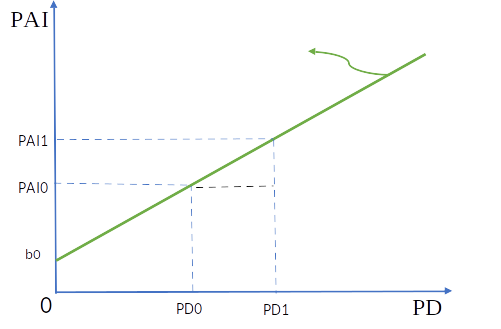
\includegraphics{20230603001915.png}

}

\end{figure}

En la gráfica, se observa una relación positiva entre las prácticas
agrícolas insostenibles (PAI) y la pérdida de diversidad (PD). A medida
que las prácticas agrícolas insostenibles aumentan, la pérdida de
biodiversidad también se incrementa. Sin embargo, la magnitud del
impacto de las prácticas agrícolas insostenibles en la pérdida de
biodiversidad se mide mediante la sensibilidad o elasticidad, que se
calcula como el cambio porcentual de las prácticas agrícolas
insostenibles dividido por el cambio porcentual en la pérdida de
diversidad.

La ecuación que representa esta relación es:

\$\$

PD = b0 + b1 * PAI

\$\$

\(↑PAI → ↑PD\): A mayor cantidad de prácticas agrícolas insostenibles,
se genera una mayor pérdida de diversidad.

Donde b1 es la sensibilidad y mide la variación de la pérdida de
biodiversidad ante cambios en las prácticas agrícolas insostenibles.

Este análisis se fundamenta en el respaldo teórico proporcionado por la
Secretaría del Convenio sobre la Diversidad Biológica (2008), que señala
cómo en las últimas cinco décadas la expansión agrícola, especialmente
en zonas tropicales y subtropicales, ha reducido significativamente los
niveles de diversidad biológica y los servicios ecosistémicos en áreas
clave, socavando así la sostenibilidad a largo plazo de la producción
agrícola en sí (p.~22).

\hypertarget{el-peruxfa-es-vulnerable-al-cambio-climuxe1tico.}{%
\section{El Perú es vulnerable al cambio
climático.}\label{el-peruxfa-es-vulnerable-al-cambio-climuxe1tico.}}

\textbf{¿Qué sectores son más vulnerables y contribuyen más a las
emisiones de gases de efecto invernadero?}

El Perú se enfrenta a la vulnerabilidad provocada por el cambio
climático, especialmente en sectores clave para el crecimiento
inclusivo. La vulnerabilidad se refiere a la sensibilidad y falta de
capacidad de respuesta y adaptación frente a los daños causados por el
cambio climático. El país presenta zonas vulnerables debido a diversas
condiciones, y aún tiene desafíos para superar la pobreza y la
desigualdad.

En 2014, las regiones más afectadas por emergencias de origen climático
fueron Amazonas, Apurímac, Cusco, Huancavelica y Pasco, concentrando más
del 63\% de las emergencias a nivel nacional. Estas situaciones exponen
a la población al riesgo de caer o mantenerse en la pobreza debido a su
vulnerabilidad frente al cambio climático.

Los sectores agrícola y pesquero, esenciales para la seguridad
alimentaria del país, dependen directamente del clima. Estos sectores
contribuyen con el 5,7\% del Producto Bruto Interno (PBI) y emplean al
25,8\% de la población económicamente activa ocupada a nivel nacional y
al 74\% de la población económicamente activa rural. Dado que el 55\% de
la población en situación de pobreza trabaja en estas actividades, queda
en evidencia la sensibilidad de un gran número de personas al cambio
climático. Además, el clima también afecta a sectores relevantes como la
minería y la energía hidroeléctrica, que dependen de los recursos
hídricos para su funcionamiento.

\begin{itemize}
\tightlist
\item
  \textbf{Sector Agrícola}
\end{itemize}

La agricultura en el Perú es vulnerable a las variaciones climáticas,
como inundaciones, granizadas, heladas y eventos del fenómeno El Niño
(ENSO), que afectan el rendimiento de los cultivos. El 34\% de la
superficie agrícola se riega y se concentra en la costa, donde hay mayor
infraestructura. El 66\% de la agricultura se desarrolla bajo secano,
dependiendo exclusivamente de las lluvias, y se encuentra principalmente
en la sierra y la selva. La sierra enfrenta deficiencias en
infraestructura de almacenamiento de agua y riego, a pesar de recibir
mayores precipitaciones. Además, la topografía accidentada limita la
disponibilidad de nuevas tierras para el cultivo. Las sequías tienen
efectos negativos significativos en esta zona. Por otro lado, la selva
experimenta altas precipitaciones durante seis meses al año, pero cuenta
con áreas limitadas propicias para la agricultura debido a restricciones
naturales.

\begin{itemize}
\tightlist
\item
  \textbf{Sector Ganadero}
\end{itemize}

El cambio climático también generará cambios importantes en el sector
ganadero, como la disminución de las áreas de pastoreo y la competencia
espacial con la agricultura. Se espera una reducción de aproximadamente
el 50\% en la extensión de los pajonales, bofedales y arbustales en la
puna, que representan el 77,6\% de la extensión total de la región. Esta
reducción afectará la capacidad de carga y la contribución relativa de
la ganadería al PBI. Además, la disminución de los bofedales, una fuente
importante de forraje durante los períodos de sequía, dificultará el
desarrollo de la ganadería, especialmente en áreas áridas donde son la
principal fuente de agua durante períodos críticos.

\begin{itemize}
\tightlist
\item
  \textbf{Sector Pesquero}
\end{itemize}

La disponibilidad de la anchoveta, recurso pesquero clave, se verá
afectada negativamente por el cambio climático, especialmente en los
escenarios RCP 8.5 y RCP 4.5. Se esperan cambios en las condiciones de
temperatura, oxígeno disuelto y productividad primaria. Esto resultará
en una disminución importante de la contribución económica del sector
pesquero a la economía nacional.

\begin{itemize}
\tightlist
\item
  \textbf{Sector Minero}
\end{itemize}

En la mayoría de las cuencas mineras, los impactos del cambio climático
en la disponibilidad hídrica no son significativos, excepto en las
cuencas mineras de cobre y zinc. La eficiencia en el uso y consumo del
agua contribuirá a reducir futuros conflictos por este recurso y
garantizar su disponibilidad para la minería, considerando que el
consumo humano y agrícola tienen prioridad legal.

\begin{itemize}
\tightlist
\item
  \textbf{Sector de Hidroenergía}
\end{itemize}

La producción eléctrica del sector de hidroenergía en el Perú está
estrechamente relacionada con la disponibilidad de agua en las cuencas.
Por lo tanto, el cambio climático puede afectar la actividad de este
sector debido a las variaciones en las condiciones de precipitación.

\begin{itemize}
\tightlist
\item
  \textbf{Sector de Infraestructura}
\end{itemize}

La infraestructura se verá afectada por eventos climáticos extremos,
especialmente relacionados con las precipitaciones. Se espera que el
aumento de lluvias genere modificaciones en los caudales de agua cerca
de las redes viales, lo que afectaría las estructuras de drenaje y
aumentaría la probabilidad de daños en las carreteras. Esto se
traduciría en un aumento en los costos de mantenimiento y reparación de
infraestructuras viales.

\begin{itemize}
\tightlist
\item
  \textbf{Sector Turismo}
\end{itemize}

El turismo es un sector importante para la economía peruana en términos
de generación de empleo, divisas, comercio e inversión. El cambio
climático afectará directamente los destinos turísticos debido a
factores como temperatura, precipitación, viento, humedad y aumento del
nivel del mar, así como eventos climáticos extremos. Estos cambios
causarán daños a la infraestructura y requerirán medidas adicionales de
emergencia, lo que aumentará los gastos en seguros, sistemas de reserva
de agua, electricidad y evacuación, afectando la competitividad, la
demanda turística, la estacionalidad y los gastos de adaptación y
mitigación.

\begin{itemize}
\tightlist
\item
  \textbf{Sector Salud}
\end{itemize}

El cambio climático representa una amenaza directa para el sector de la
salud y la economía en general. Puede afectar directamente a la
población al modificar la frecuencia y distribución de enfermedades
transmitidas por vectores, como la malaria, y también puede tener
efectos indirectos al empeorar la economía de los hogares.

En cuanto a las emisiones de gases de efecto invernadero, no todos los
sectores productivos contribuyen de la misma manera. Según el Panel
Intergubernamental sobre el Cambio Climático, los principales emisores a
nivel mundial son la generación de electricidad, las actividades
agropecuarias y la industria.

\begin{figure}

\caption{\label{fig-2}Relación entre las prácticas agrícolas
insostenibles y la pérdida de biodiversidad}

{\centering 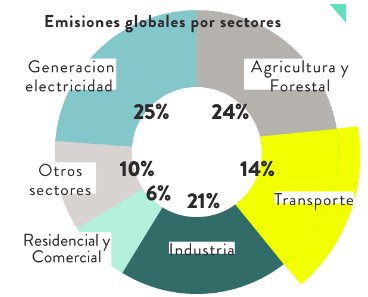
\includegraphics{20230603083843.png}

}

\end{figure}

Nota: Prevencionintegral\&ORP

\textbf{Se manifiesta que la fijación de precios y la regulación son los
principales instrumentos para promover el uso sostenible de los Recursos
Naturales.}

La fijación de precios y la regulación son herramientas fundamentales
utilizadas para promover el uso sostenible de los recursos naturales.
Estas políticas ambientales buscan reducir la degradación del medio
ambiente al costo social más bajo posible. Un enfoque clave para lograr
este objetivo es alinear los costos privados con los costos sociales, de
manera que las externalidades sean consideradas en la toma de
decisiones.

En los últimos años, se ha acumulado evidencia que respalda la
efectividad de los instrumentos económicos para mejorar la calidad
ambiental y fomentar la sostenibilidad de los recursos naturales. Estos
instrumentos económicos pueden generar beneficios significativos, como
la reducción de los costos de cumplimiento para las industrias, la
disminución de las cargas administrativas en el sector público, la
mejora de las condiciones ambientales y la promoción de la salud humana.
A su vez, esto contribuye a mejorar la productividad económica y reducir
los gastos en atención médica.

En el contexto legal, la legislación ambiental en el Perú se basa en la
Constitución Política de 1993, que garantiza a todas las personas el
derecho a disfrutar de un medio ambiente seguro y adecuado para su
sustento. En este marco, se ha incorporado el principio del ``usuario
pagador'' en la legislación, que establece que aquellos que utilizan los
recursos naturales tienen la responsabilidad de pagar por su uso. Este
principio se encuentra explícitamente incluido en la Ley Orgánica para
el Aprovechamiento Sostenible de los Recursos Naturales.

Sin embargo, en la práctica, la implementación del principio del
``contaminador pagador'' en relación con el control y prevención de la
contaminación en sectores industriales presenta desafíos y limitaciones.
Aunque existen políticas de precios y regulaciones establecidas, su
aplicación efectiva aún requiere mejoras para garantizar un cumplimiento
adecuado y promover un mayor control de la contaminación en el sector
industrial.

\hypertarget{anuxe1lisis-de-las-exportaciones-de-productos-tradicionales-precios-del-petruxf3leo-crudo-y-derivados-y-precios-del-gas-natural-durante-el-periodo-enero-2012---mayo-2022}{%
\section{Análisis de las exportaciones de productos tradicionales,
precios del petróleo crudo y derivados, y precios del gas natural
durante el periodo enero 2012 - mayo
2022}\label{anuxe1lisis-de-las-exportaciones-de-productos-tradicionales-precios-del-petruxf3leo-crudo-y-derivados-y-precios-del-gas-natural-durante-el-periodo-enero-2012---mayo-2022}}

En este análisis, examinaremos tanto las exportaciones de productos
tradicionales como los precios del petróleo crudo y derivados, y los
precios del gas natural de forma individual y conjunta durante el
periodo comprendido entre enero de 2012 y mayo de 2022.

\hypertarget{anuxe1lisis-individual-de-las-series}{%
\subsection{Análisis individual de las
series}\label{anuxe1lisis-individual-de-las-series}}

\hypertarget{anuxe1lisis-de-los-gruxe1ficos}{%
\subsubsection{Análisis de los
gráficos}\label{anuxe1lisis-de-los-gruxe1ficos}}

La Figura~\ref{fig-3} muestra las exportaciones de productos
tradicionales en comparación con los precios del petróleo crudo y
derivados (en dólares estadounidenses por barril).

\begin{figure}

\caption{\label{fig-3}Exportaciones de productos tradicionales y precios
del petróleo crudo y derivados}

{\centering 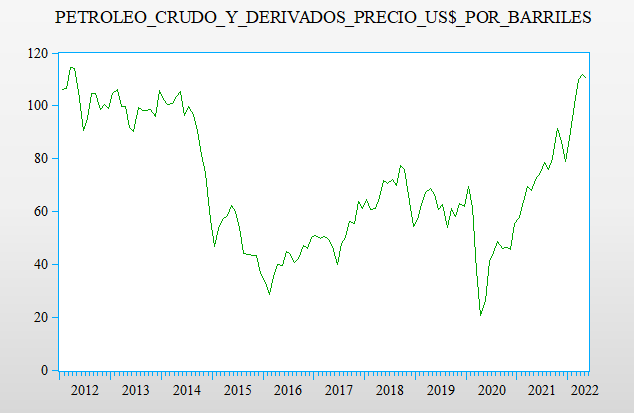
\includegraphics{20230603085638.png}

}

\end{figure}

\emph{Nota: Fuente: BCRP (14 de julio de 2022). Elaboración propia.}

\textbf{Interpretación:} La serie de precios del petróleo crudo y
derivados muestra un comportamiento con cambios bruscos y repentinos
durante casi todo el periodo analizado, con valores atípicos destacados
en los años 2014, 2015, 2020 y 2022. Esto sugiere que la serie exhibe
una variación aleatoria en su comportamiento.

La caída de los precios del petróleo entre mediados de 2014 y principios
de 2015 se debió principalmente a factores relacionados con la oferta,
como el aumento de la producción de petróleo en Estados Unidos, la
disminución de las tensiones geopolíticas y los cambios en las políticas
de la OPEP. Esta caída del precio del petróleo también afectó
negativamente las previsiones de demanda de petróleo durante mediados de
2015 y principios de 2016.

En el año 2017, se observó un aumento en el interés de las empresas
internacionales por la exploración y explotación de petróleo en aguas
profundas (offshore), debido al potencial de reservas de petróleo. Esto
resultó en un incremento de los precios del petróleo entre 2017 y 2018.

En 2022, se produjo un fuerte aumento en los precios del petróleo debido
a la situación crítica que enfrentaba Europa y a las políticas
establecidas para reducir la dependencia de los suministros rusos. Del
25 de mayo al 1 de junio de 2022, el precio del petróleo aumentó un
2,1\%, alcanzando los 115,3 dólares por barril. Este incremento reflejó
la señal de una menor oferta y una creciente demanda antes de la
temporada alta de conducción de verano en Estados Unidos y Europa. En
mayo, el precio del petróleo subió un 9,4\%.

La Figura~\ref{fig-4} muestra las exportaciones de productos
tradicionales en relación con los precios del gas natural (en dólares
estadounidenses por metro cúbico).

\begin{figure}

\caption{\label{fig-4}Exportaciones de productos tradicionales y precios
del gas natural}

{\centering 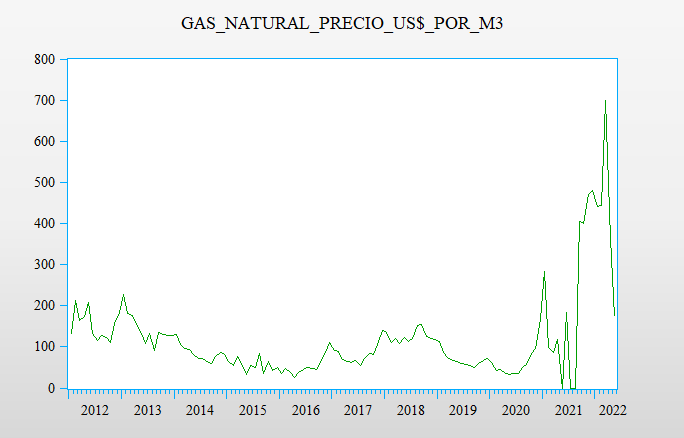
\includegraphics{20230603090113.png}

}

\end{figure}

\emph{Nota: Fuente: BCRP (14 de julio de 2022). Elaboración propia.}

\textbf{Interpretación:} La serie de precios del gas natural presenta
valores atípicos en los años 2021 y 2022, con cambios bruscos más
pronunciados durante esos mismos años. Además, se observa un patrón
cíclico en el periodo comprendido entre 2012 y 2020, seguido de una
variación aleatoria en los últimos años.

A partir de 2019 y 2020, el precio del gas natural se redujo debido a la
``revolución'' del gas de fracking en Estados Unidos. Sin embargo, en
julio y agosto de 2020, los precios del gas se vieron afectados por la
crisis del Covid-19.

A finales de 2020, se reactivó la demanda de gas natural, pero la oferta
no pudo mantenerse al ritmo necesario, lo que generó retrasos en la
respuesta a la demanda, principalmente debido a problemas logísticos
relacionados con el transporte de gas. Además, el invierno prolongado
agotó las reservas en el hemisferio norte. Asia fue responsable del 70\%
del consumo global de gas natural y pagó precios elevados. Europa
también experimentó un déficit de suministro a finales de 2020,
situación que se prolongó a lo largo de 2021.

En septiembre de 2021, el precio del gas natural aumentó debido a que la
producción mundial de gas no creció al mismo ritmo que la demanda, lo
que provocó un incremento en el precio. Los niveles de almacenamiento en
los 48 estados inferiores de EE. UU. se encontraban ligeramente por
debajo de lo normal, según la Administración de Información Energética.
Esta situación se vio agravada por el huracán Ida, que interrumpió la
producción en Noruega y Rusia, así como en el Golfo de México, donde
gran parte de la producción de petróleo y gas quedó fuera de servicio.

En abril de 2022, la producción de hidrocarburos experimentó un
crecimiento interanual del 26,2\%, impulsado por una mayor extracción de
todos sus componentes (hidrocarburos líquidos y gas natural) desde 2021.
En el periodo de enero a abril, el sector se expandió un 15,0\%.

\hypertarget{anuxe1lisis-de-normalidad-de-las-series}{%
\subsubsection{Análisis de normalidad de las
series}\label{anuxe1lisis-de-normalidad-de-las-series}}

La Figura~\ref{fig-5} muestra los resultados de la prueba de normalidad
aplicada al precio del Petróleo crudo y derivados.

\begin{figure}

\caption{\label{fig-5}Prueba de normalidad del precio del Petróleo crudo
y derivados}

{\centering 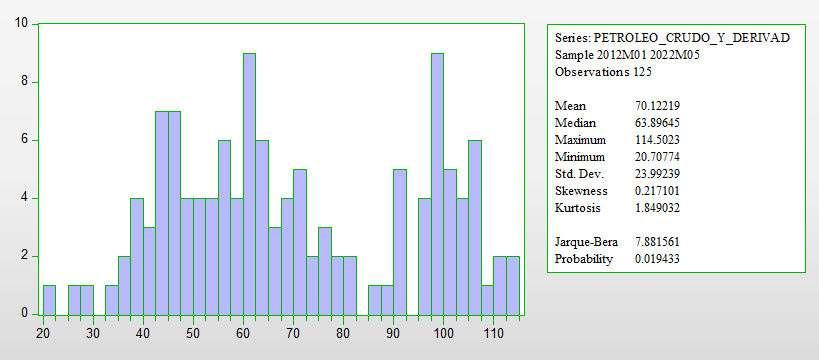
\includegraphics{20230603090708.png}

}

\end{figure}

\emph{Nota: Elaboración propia.}

\textbf{Interpretación:} En cuanto a la prueba de normalidad, se observa
que la serie del precio del Petróleo crudo y derivados presenta una
cercanía entre la media y la mediana. Además, el coeficiente de
asimetría (skewness=0.217) tiende a cero y la kurtosis tiende débilmente
a 3, lo cual sugiere que la distribución podría ser normal.

Sin embargo, para realizar un análisis más riguroso, se utiliza el
estadístico de Jarque-Bera bajo la hipótesis nula de que la serie sigue
una distribución normal. En este caso, el valor de JB es 7.88, que es
mayor que el valor crítico de 5.99, lo que nos lleva a rechazar la
hipótesis nula de normalidad. Además, la probabilidad asociada al valor
de JB es 0.019, que es menor al nivel de significancia del 5\%, lo que
confirma que la serie no sigue una distribución normal.

Para corregir la falta de normalidad, se aplica una transformación
logarítmica a la serie del Petróleo crudo y derivados.

La Figura~\ref{fig-6} muestra la serie del precio del Petróleo crudo y
derivados después de aplicar la transformación logarítmica para corregir
la falta de normalidad.

\begin{figure}

\caption{\label{fig-6}Corrección de normalidad del precio del Petróleo
crudo y derivados}

{\centering 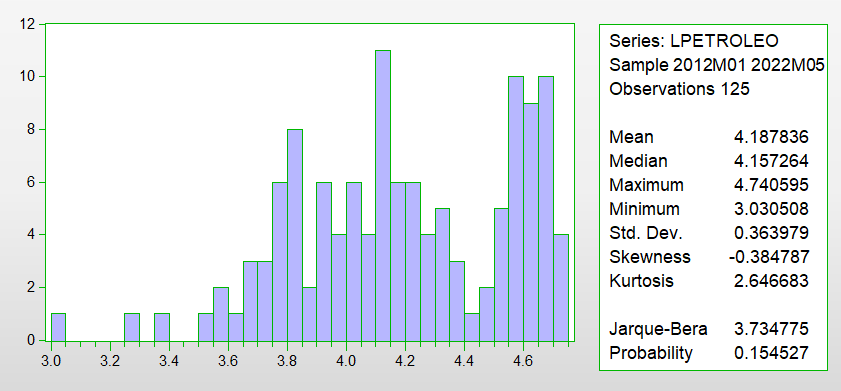
\includegraphics{20230603090807.png}

}

\end{figure}

\emph{Nota: Elaboración propia.}

\textbf{Interpretación:} Al aplicar la transformación logarítmica a la
serie del Petróleo crudo y derivados, se observa que se corrige la falta
de normalidad. El estadístico de Jarque-Bera es 3.73, que es menor que
el valor crítico de 5.99, lo que nos lleva a aceptar la hipótesis nula
de normalidad. Además, la probabilidad asociada al valor de JB es 0.155,
que es mayor al nivel de significancia del 5\%, lo que confirma que la
serie sigue una distribución normal después de la transformación
logarítmica.

La Figura~\ref{fig-7} muestra los resultados de la prueba de normalidad
aplicada al precio del Gas natural.

\begin{figure}

\caption{\label{fig-7}Prueba de normalidad del precio del Gas natural}

{\centering 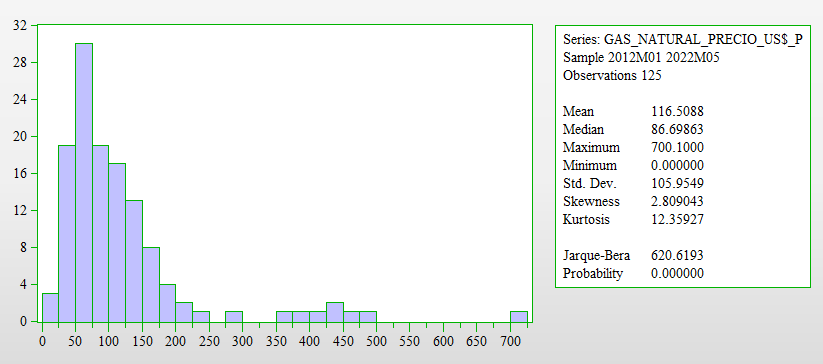
\includegraphics{20230603091227.png}

}

\end{figure}

\emph{Nota: Elaboración propia.}

\textbf{Interpretación:} Según la prueba de normalidad, la serie del
precio del Gas natural presenta poca cercanía entre la media y la
mediana. Además, el coeficiente de asimetría (skewness=2.809) no tiende
a cero y la kurtosis es 12.36, lo cual indica que la distribución se
aleja de una distribución normal. Para realizar un análisis más
riguroso, se utiliza el estadístico de Jarque-Bera bajo la hipótesis
nula de que la serie sigue una distribución normal. En este caso, el
valor de JB es 620.619, que es mayor que el valor crítico de 5.99, lo
que nos lleva a rechazar la hipótesis nula de normalidad. Además, la
probabilidad asociada al valor de JB es 0.000, que es menor al nivel de
significancia del 5\%, confirmando que la serie no sigue una
distribución normal.

La Figura~\ref{fig-8} muestra la serie del precio del Gas natural
después de aplicar una transformación para corregir la falta de
normalidad.

\begin{figure}

\caption{\label{fig-8}Corrección de normalidad del precio del Gas
natural}

{\centering 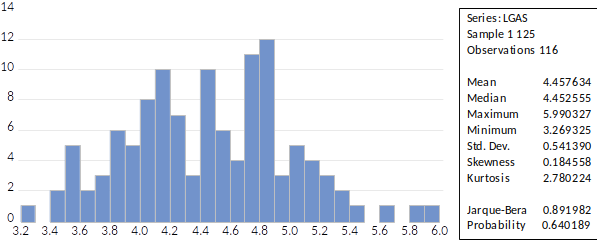
\includegraphics{20230603091315.png}

}

\end{figure}

\emph{Nota: Elaboración propia.}

\textbf{Interpretación:} Al aplicar la transformación de datos, se logra
una distribución normal en los precios del Gas natural. La
transformación se realiza utilizando la media y la desviación estándar
de la distribución, y se reemplazan los valores atípicos y extremos con
valores nulos o perdidos en el sistema. Se observa que el estadístico de
Jarque-Bera es 0.89, que es menor que el valor crítico de 5.99, lo que
nos permite aceptar la hipótesis nula de presencia de una distribución
normal. Además, la probabilidad asociada al valor de JB es 0.64, que es
mayor al nivel de significancia del 5\%, lo que confirma que la serie de
precios del Gas natural sigue una distribución normal después de la
transformación.

\hypertarget{anuxe1lisis-conjunta-de-las-series}{%
\subsection{Análisis conjunta de las
series}\label{anuxe1lisis-conjunta-de-las-series}}

La Figura~\ref{fig-9} muestra la evolución del precio del petróleo y el
gas en dólares.

\begin{figure}

\caption{\label{fig-9}Evolución del precio del petróleo y gas (en
dólares)}

{\centering 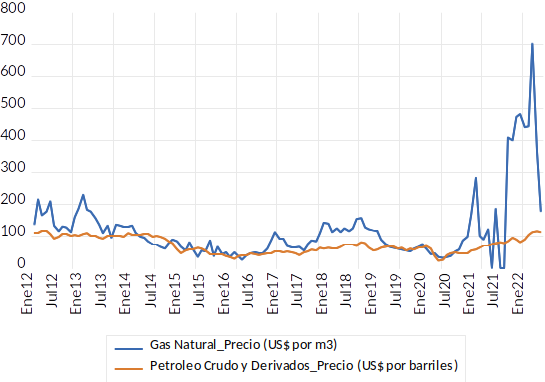
\includegraphics{20230603091833.png}

}

\end{figure}

\emph{\textbf{Nota:} Datos obtenidos del BCRP y gráfico elaborado por
nosotros.}

\textbf{Interpretación:} El incremento de los precios del petróleo y el
gas en esta visualización se debe a la guerra en Ucrania y los temores
sobre el suministro de materias primas provenientes de Rusia. El precio
del petróleo alcanzó su máximo en casi diez años, mientras que el gas
natural alcanzó récords históricos.

Las tensiones geopolíticas internacionales y el encarecimiento del
petróleo fueron factores clave para el aumento en los precios del gas.
Sin embargo, este aumento también ha tenido un impacto negativo en los
alimentos y el costo de vida de las familias más pobres, lo que plantea
un desafío para el gobierno.

La Figura~\ref{fig-10} muestra un análisis de caja y bigote del precio
de gas y petróleo.

\begin{figure}

\caption{\label{fig-10}Análisis de caja y bigote del precio de gas y
petróleo}\begin{minipage}[t]{0.50\linewidth}
\subcaption{\label{fig-10.1}Surus}

{\centering 

\raisebox{-\height}{

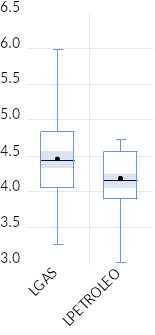
\includegraphics{20230603091856.png}

}

}

\end{minipage}%
%
\begin{minipage}[t]{0.50\linewidth}
\subcaption{\label{fig-10.2}Hanno}

{\centering 

\raisebox{-\height}{

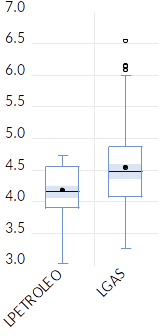
\includegraphics{20230603091845.png}

}

}

\end{minipage}%

\end{figure}

\emph{\textbf{Nota:} Datos obtenidos del BCRP y gráfico elaborado por
nosotros.}

\textbf{Interpretación:} En el gráfico de la izquierda, se observa que
tanto el precio del gas natural como el precio del petróleo tienen
rangos normales, lo que indica que los datos están concentrados dentro
de esos rangos. Además, el precio del gas natural muestra una
distribución simétrica, ya que la línea de la mediana está cerca del
centro de la caja. Sin embargo, se presentan algunos datos atípicos.

En el gráfico de la derecha, utilizando una transformación de datos, se
logra una distribución normal en los precios del gas. La distribución se
crea utilizando la media y la desviación estándar de la distribución de
gas. En esta distribución, las líneas de la mediana y la media se
superponen, los rangos intercuartílicos (representados por los bigotes)
y las cajas son de tamaño similar, y los datos atípicos son poco
comunes.

En cuanto al precio del petróleo, también muestra una distribución
simétrica, ya que la mediana está cerca del centro de la caja. En esta
distribución, la media es similar a la mediana, lo que indica una
distribución normal.

La Figura~\ref{fig-11} muestra un gráfico de dispersión que representa
la relación entre el precio del gas y el precio del petróleo.

\begin{figure}

\caption{\label{fig-11}Gráfico de dispersión de las variables precio de
gas y precio de petróleo}

{\centering 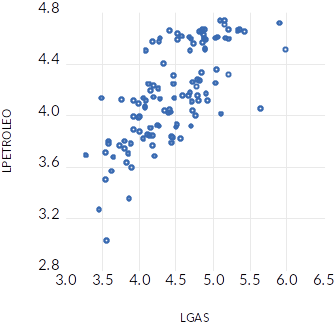
\includegraphics{20230603091904.png}

}

\end{figure}

\emph{\textbf{Nota:} Datos obtenidos del BCRP y gráfico elaborado por
nosotros.}

\textbf{Interpretación:} En el gráfico, se puede observar una relación
lineal positiva moderada entre el precio del petróleo y el precio del
gas. A medida que el precio del petróleo aumenta, el precio del gas
también tiende a aumentar.

La Tabla 2 muestra los resultados de la regresión entre el precio del
petróleo y el precio del gas.

\begin{figure}

\caption{Tabla 2: Regresión de precio de petróleo y precio del gas}

{\centering 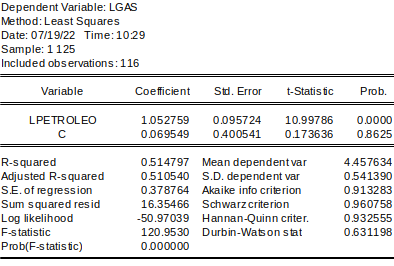
\includegraphics{20230603100307.png}

}

\end{figure}

\emph{\textbf{Nota:} Datos obtenidos del BCRP.}

El valor P \textless{} 0.05 en el análisis de regresión indica que el
precio del petróleo que estamos analizando es significativo y tiene una
relación con el precio del gas.

Además, el coeficiente R-Sq (adj) nos indica que el 51\% de la variación
en el precio del gas se explica por el precio del petróleo.

La ecuación de regresión muestra que, por cada aumento en el precio del
petróleo, el precio del gas aumenta en 1.0527 dólares.

\hypertarget{relaciuxf3n-entre-el-volumen-del-cobre-miles-de-toneladas-y-el-oro-miles-de-onzas-troy.}{%
\section{Relación entre el volumen del cobre (miles de toneladas) y el
oro (miles de onzas
troy).}\label{relaciuxf3n-entre-el-volumen-del-cobre-miles-de-toneladas-y-el-oro-miles-de-onzas-troy.}}

Para analizar la relación entre el volumen del cobre (medido en miles de
toneladas) y el oro (medido en miles de onzas troy), consideramos las
series mensuales de exportaciones de productos tradicionales del BCRP.
Graficaremos y explicaremos su comportamiento, evaluando si existe una
relación de largo plazo (cointegración) entre ambas variables en el
Perú, utilizando el mismo período que en las preguntas anteriores
(mencionar el período específico). \$\$


\printbibliography


\end{document}
